\documentclass[1p]{elsarticle_modified}
%\bibliographystyle{elsarticle-num}

%\usepackage[colorlinks]{hyperref}
%\usepackage{abbrmath_seonhwa} %\Abb, \Ascr, \Acal ,\Abf, \Afrak
\usepackage{amsfonts}
\usepackage{amssymb}
\usepackage{amsmath}
\usepackage{amsthm}
\usepackage{scalefnt}
\usepackage{amsbsy}
\usepackage{kotex}
\usepackage{caption}
\usepackage{subfig}
\usepackage{color}
\usepackage{graphicx}
\usepackage{xcolor} %% white, black, red, green, blue, cyan, magenta, yellow
\usepackage{float}
\usepackage{setspace}
\usepackage{hyperref}

\usepackage{tikz}
\usetikzlibrary{arrows}

\usepackage{multirow}
\usepackage{array} % fixed length table
\usepackage{hhline}

%%%%%%%%%%%%%%%%%%%%%
\makeatletter
\renewcommand*\env@matrix[1][\arraystretch]{%
	\edef\arraystretch{#1}%
	\hskip -\arraycolsep
	\let\@ifnextchar\new@ifnextchar
	\array{*\c@MaxMatrixCols c}}
\makeatother %https://tex.stackexchange.com/questions/14071/how-can-i-increase-the-line-spacing-in-a-matrix
%%%%%%%%%%%%%%%

\usepackage[normalem]{ulem}

\newcommand{\msout}[1]{\ifmmode\text{\sout{\ensuremath{#1}}}\else\sout{#1}\fi}
%SOURCE: \msout is \stkout macro in https://tex.stackexchange.com/questions/20609/strikeout-in-math-mode

\newcommand{\cancel}[1]{
	\ifmmode
	{\color{red}\msout{#1}}
	\else
	{\color{red}\sout{#1}}
	\fi
}

\newcommand{\add}[1]{
	{\color{blue}\uwave{#1}}
}

\newcommand{\replace}[2]{
	\ifmmode
	{\color{red}\msout{#1}}{\color{blue}\uwave{#2}}
	\else
	{\color{red}\sout{#1}}{\color{blue}\uwave{#2}}
	\fi
}

\newcommand{\Sol}{\mathcal{S}} %segment
\newcommand{\D}{D} %diagram
\newcommand{\A}{\mathcal{A}} %arc


%%%%%%%%%%%%%%%%%%%%%%%%%%%%%5 test

\def\sl{\operatorname{\textup{SL}}(2,\Cbb)}
\def\psl{\operatorname{\textup{PSL}}(2,\Cbb)}
\def\quan{\mkern 1mu \triangleright \mkern 1mu}

\theoremstyle{definition}
\newtheorem{thm}{Theorem}[section]
\newtheorem{prop}[thm]{Proposition}
\newtheorem{lem}[thm]{Lemma}
\newtheorem{ques}[thm]{Question}
\newtheorem{cor}[thm]{Corollary}
\newtheorem{defn}[thm]{Definition}
\newtheorem{exam}[thm]{Example}
\newtheorem{rmk}[thm]{Remark}
\newtheorem{alg}[thm]{Algorithm}

\newcommand{\I}{\sqrt{-1}}
\begin{document}

%\begin{frontmatter}
%
%\title{Boundary parabolic representations of knots up to 8 crossings}
%
%%% Group authors per affiliation:
%\author{Yunhi Cho} 
%\address{Department of Mathematics, University of Seoul, Seoul, Korea}
%\ead{yhcho@uos.ac.kr}
%
%
%\author{Seonhwa Kim} %\fnref{s_kim}}
%\address{Center for Geometry and Physics, Institute for Basic Science, Pohang, 37673, Korea}
%\ead{ryeona17@ibs.re.kr}
%
%\author{Hyuk Kim}
%\address{Department of Mathematical Sciences, Seoul National University, Seoul 08826, Korea}
%\ead{hyukkim@snu.ac.kr}
%
%\author{Seokbeom Yoon}
%\address{Department of Mathematical Sciences, Seoul National University, Seoul, 08826,  Korea}
%\ead{sbyoon15@snu.ac.kr}
%
%\begin{abstract}
%We find all boundary parabolic representation of knots up to 8 crossings.
%
%\end{abstract}
%\begin{keyword}
%    \MSC[2010] 57M25 
%\end{keyword}
%
%\end{frontmatter}

%\linenumbers
%\tableofcontents
%
\newcommand\colored[1]{\textcolor{white}{\rule[-0.35ex]{0.8em}{1.4ex}}\kern-0.8em\color{red} #1}%
%\newcommand\colored[1]{\textcolor{white}{ #1}\kern-2.17ex	\textcolor{white}{ #1}\kern-1.81ex	\textcolor{white}{ #1}\kern-2.15ex\color{red}#1	}

{\Large $\underline{12a_{0215}~(K12a_{0215})}$}

\setlength{\tabcolsep}{10pt}
\renewcommand{\arraystretch}{1.6}
\vspace{1cm}\begin{tabular}{m{100pt}>{\centering\arraybackslash}m{274pt}}
\multirow{5}{120pt}{
	\centering
	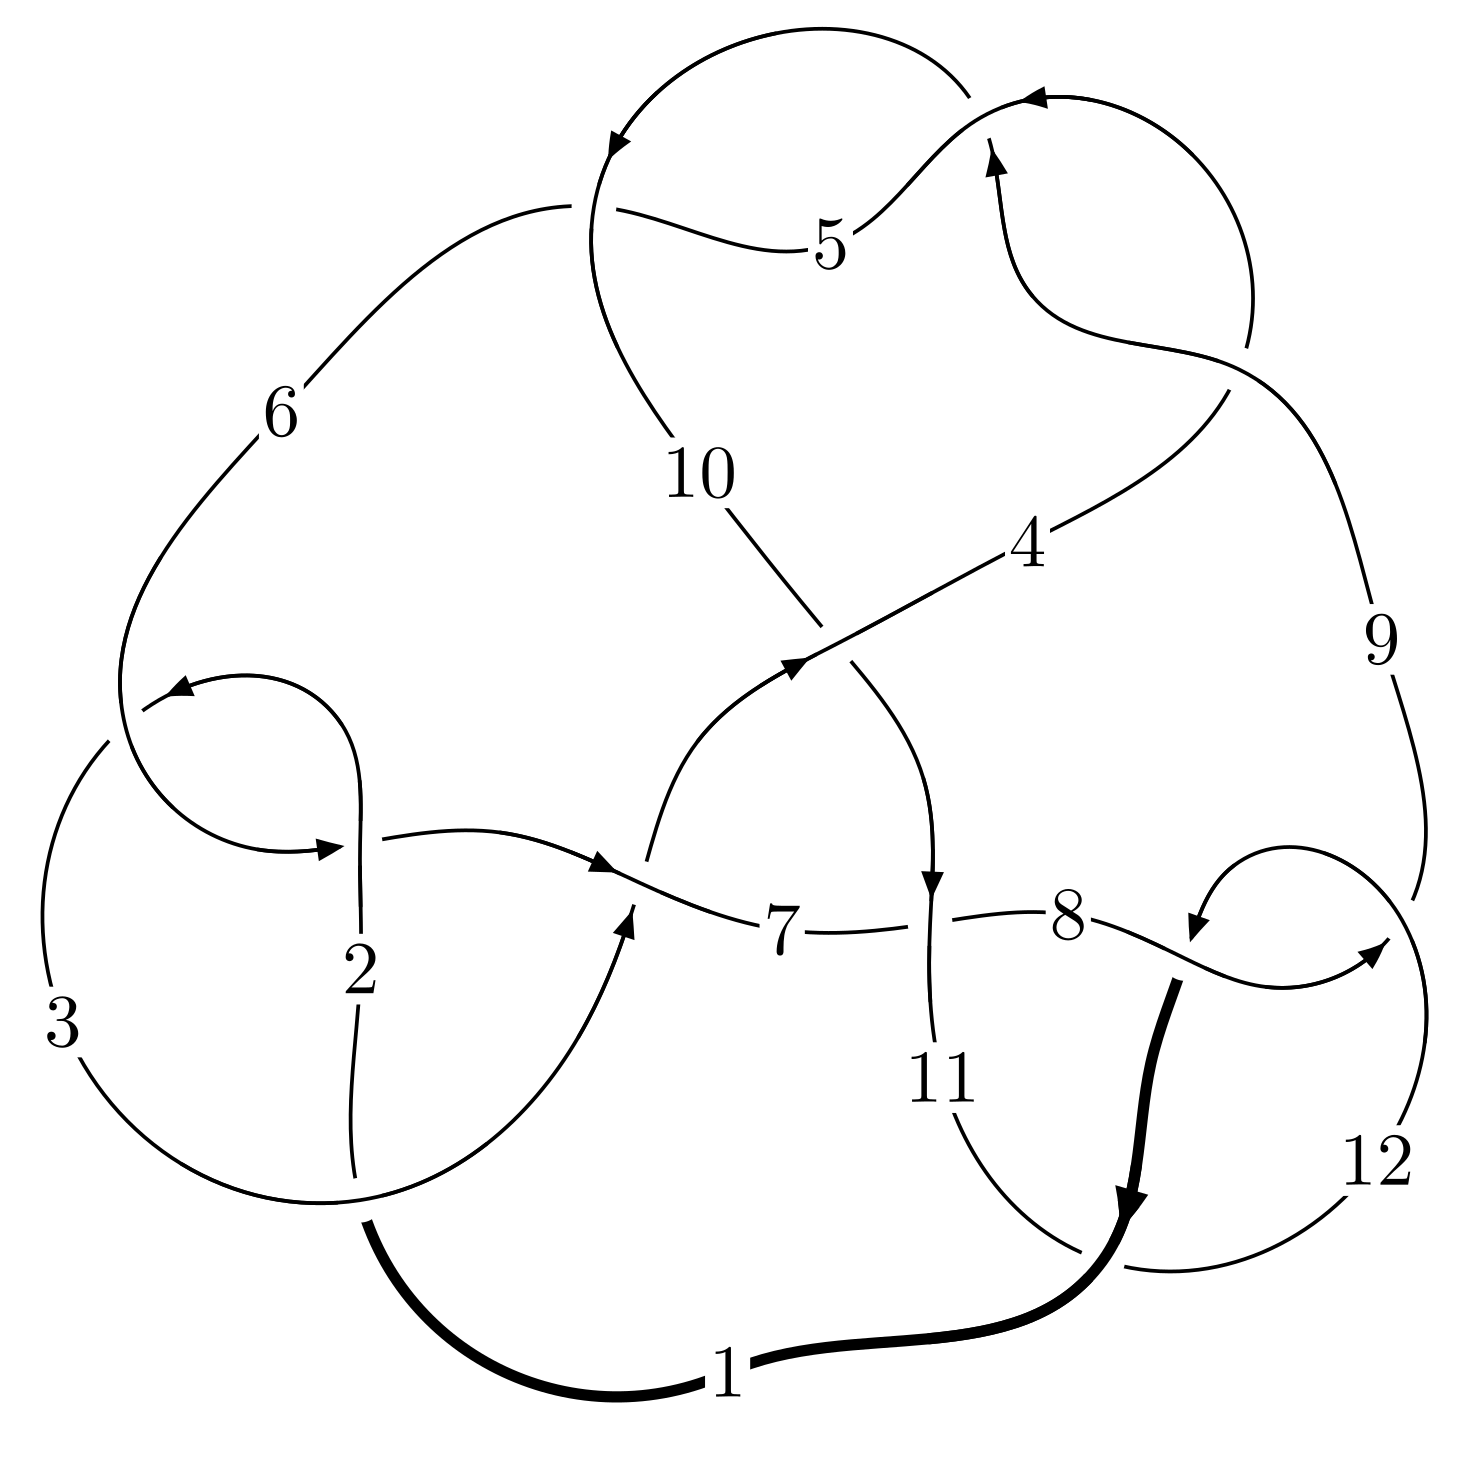
\includegraphics[width=112pt]{../../../GIT/diagram.site/Diagrams/png/1016_12a_0215.png}\\
\ \ \ A knot diagram\footnotemark}&
\allowdisplaybreaks
\textbf{Linearized knot diagam} \\
\cline{2-2}
 &
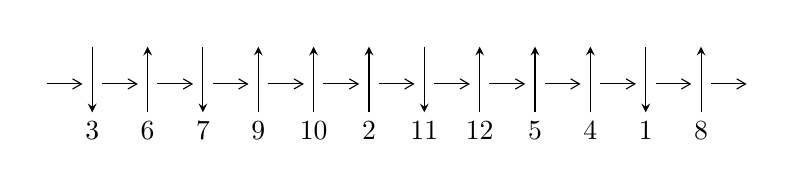
\begin{tikzpicture}[x=20pt, y=17pt]
	% nodes
	\node (C0) at (0, 0) {};
	\node (C1) at (1, 0) {};
	\node (C1U) at (1, +1) {};
	\node (C1D) at (1, -1) {3};

	\node (C2) at (2, 0) {};
	\node (C2U) at (2, +1) {};
	\node (C2D) at (2, -1) {6};

	\node (C3) at (3, 0) {};
	\node (C3U) at (3, +1) {};
	\node (C3D) at (3, -1) {7};

	\node (C4) at (4, 0) {};
	\node (C4U) at (4, +1) {};
	\node (C4D) at (4, -1) {9};

	\node (C5) at (5, 0) {};
	\node (C5U) at (5, +1) {};
	\node (C5D) at (5, -1) {10};

	\node (C6) at (6, 0) {};
	\node (C6U) at (6, +1) {};
	\node (C6D) at (6, -1) {2};

	\node (C7) at (7, 0) {};
	\node (C7U) at (7, +1) {};
	\node (C7D) at (7, -1) {11};

	\node (C8) at (8, 0) {};
	\node (C8U) at (8, +1) {};
	\node (C8D) at (8, -1) {12};

	\node (C9) at (9, 0) {};
	\node (C9U) at (9, +1) {};
	\node (C9D) at (9, -1) {5};

	\node (C10) at (10, 0) {};
	\node (C10U) at (10, +1) {};
	\node (C10D) at (10, -1) {4};

	\node (C11) at (11, 0) {};
	\node (C11U) at (11, +1) {};
	\node (C11D) at (11, -1) {1};

	\node (C12) at (12, 0) {};
	\node (C12U) at (12, +1) {};
	\node (C12D) at (12, -1) {8};
	\node (C13) at (13, 0) {};

	% arrows
	\draw[->,>={angle 60}]
	(C0) edge (C1) (C1) edge (C2) (C2) edge (C3) (C3) edge (C4) (C4) edge (C5) (C5) edge (C6) (C6) edge (C7) (C7) edge (C8) (C8) edge (C9) (C9) edge (C10) (C10) edge (C11) (C11) edge (C12) (C12) edge (C13) ;	\draw[->,>=stealth]
	(C1U) edge (C1D) (C2D) edge (C2U) (C3U) edge (C3D) (C4D) edge (C4U) (C5D) edge (C5U) (C6D) edge (C6U) (C7U) edge (C7D) (C8D) edge (C8U) (C9D) edge (C9U) (C10D) edge (C10U) (C11U) edge (C11D) (C12D) edge (C12U) ;
	\end{tikzpicture} \\
\hhline{~~} \\& 
\textbf{Solving Sequence} \\ \cline{2-2} 
 &
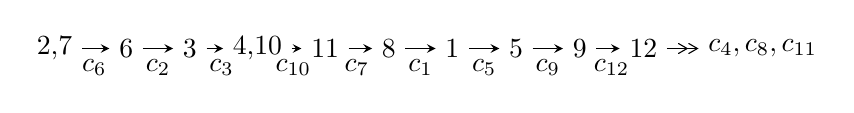
\begin{tikzpicture}[x=23pt, y=7pt]
	% node
	\node (A0) at (-1/8, 0) {2,7};
	\node (A1) at (1, 0) {6};
	\node (A2) at (2, 0) {3};
	\node (A3) at (49/16, 0) {4,10};
	\node (A4) at (33/8, 0) {11};
	\node (A5) at (41/8, 0) {8};
	\node (A6) at (49/8, 0) {1};
	\node (A7) at (57/8, 0) {5};
	\node (A8) at (65/8, 0) {9};
	\node (A9) at (73/8, 0) {12};
	\node (C1) at (1/2, -1) {$c_{6}$};
	\node (C2) at (3/2, -1) {$c_{2}$};
	\node (C3) at (5/2, -1) {$c_{3}$};
	\node (C4) at (29/8, -1) {$c_{10}$};
	\node (C5) at (37/8, -1) {$c_{7}$};
	\node (C6) at (45/8, -1) {$c_{1}$};
	\node (C7) at (53/8, -1) {$c_{5}$};
	\node (C8) at (61/8, -1) {$c_{9}$};
	\node (C9) at (69/8, -1) {$c_{12}$};
	\node (A10) at (11, 0) {$c_{4},c_{8},c_{11}$};

	% edge
	\draw[->,>=stealth]	
	(A0) edge (A1) (A1) edge (A2) (A2) edge (A3) (A3) edge (A4) (A4) edge (A5) (A5) edge (A6) (A6) edge (A7) (A7) edge (A8) (A8) edge (A9) ;
	\draw[->>,>={angle 60}]	
	(A9) edge (A10);
\end{tikzpicture} \\ 

\end{tabular} \\

\footnotetext{
The image of knot diagram is generated by the software ``\textbf{Draw programme}" developed by Andrew Bartholomew(\url{http://www.layer8.co.uk/maths/draw/index.htm\#Running-draw}), where we modified some parts for our purpose(\url{https://github.com/CATsTAILs/LinksPainter}).
}\phantom \\ \newline 
\centering \textbf{Ideals for irreducible components\footnotemark of $X_{\text{par}}$} 
 
\begin{align*}
I^u_{1}&=\langle 
- u^{25}+u^{24}+\cdots+2 b+1,\;u^{25}- u^{24}+\cdots+2 a-1,\;u^{27}- u^{26}+\cdots+2 u-1\rangle \\
I^u_{2}&=\langle 
-8.39891\times10^{38} u^{81}+2.15045\times10^{38} u^{80}+\cdots+2.93276\times10^{39} b-1.22548\times10^{40},\\
\phantom{I^u_{2}}&\phantom{= \langle  }2.50222\times10^{40} u^{81}-4.66705\times10^{40} u^{80}+\cdots+2.05293\times10^{40} a-7.74216\times10^{40},\;u^{82}-2 u^{81}+\cdots-19 u+7\rangle \\
I^u_{3}&=\langle 
b+a+u,\;a^2-2 a-2 u+1,\;u^2+u+1\rangle \\
I^u_{4}&=\langle 
b+u-1,\;a+1,\;u^2- u+1\rangle \\
I^u_{5}&=\langle 
b+a+1,\;a^2+2 a u+2 a- u,\;u^2+u+1\rangle \\
I^u_{6}&=\langle 
b- u,\;a+u-1,\;u^2- u+1\rangle \\
\\
\end{align*}
\raggedright * 6 irreducible components of $\dim_{\mathbb{C}}=0$, with total 121 representations.\\
\footnotetext{All coefficients of polynomials are rational numbers. But the coefficients are sometimes approximated in decimal forms when there is not enough margin.}
\newpage
\renewcommand{\arraystretch}{1}
\centering \section*{I. $I^u_{1}= \langle - u^{25}+u^{24}+\cdots+2 b+1,\;u^{25}- u^{24}+\cdots+2 a-1,\;u^{27}- u^{26}+\cdots+2 u-1 \rangle$}
\flushleft \textbf{(i) Arc colorings}\\
\begin{tabular}{m{7pt} m{180pt} m{7pt} m{180pt} }
\flushright $a_{2}=$&$\begin{pmatrix}0\\u\end{pmatrix}$ \\
\flushright $a_{7}=$&$\begin{pmatrix}1\\0\end{pmatrix}$ \\
\flushright $a_{6}=$&$\begin{pmatrix}1\\u^2\end{pmatrix}$ \\
\flushright $a_{3}=$&$\begin{pmatrix}u\\u^3+u\end{pmatrix}$ \\
\flushright $a_{4}=$&$\begin{pmatrix}- u^3\\u^3+u\end{pmatrix}$ \\
\flushright $a_{10}=$&$\begin{pmatrix}-\frac{1}{2} u^{25}+\frac{1}{2} u^{24}+\cdots-2 u+\frac{1}{2}\\\frac{1}{2} u^{25}-\frac{1}{2} u^{24}+\cdots+2 u-\frac{1}{2}\end{pmatrix}$ \\
\flushright $a_{11}=$&$\begin{pmatrix}-\frac{1}{2} u^{23}+\frac{1}{2} u^{22}+\cdots-2 u+\frac{1}{2}\\u^3+u\end{pmatrix}$ \\
\flushright $a_{8}=$&$\begin{pmatrix}-\frac{1}{2} u^{26}+\frac{1}{2} u^{25}+\cdots+\frac{1}{2} u+1\\u^6+2 u^4+u^2\end{pmatrix}$ \\
\flushright $a_{1}=$&$\begin{pmatrix}u^3\\u^5+u^3+u\end{pmatrix}$ \\
\flushright $a_{5}=$&$\begin{pmatrix}-\frac{1}{2} u^{26}-3 u^{24}+\cdots-2 u+\frac{3}{2}\\\frac{1}{2} u^{25}-\frac{1}{2} u^{24}+\cdots+2 u-\frac{1}{2}\end{pmatrix}$ \\
\flushright $a_{9}=$&$\begin{pmatrix}\frac{1}{2} u^{26}-\frac{1}{2} u^{25}+\cdots-\frac{1}{2} u^3-1\\- u^8-2 u^6-2 u^4\end{pmatrix}$ \\
\flushright $a_{12}=$&$\begin{pmatrix}-\frac{1}{2} u^{23}+\frac{1}{2} u^{22}+\cdots-2 u+\frac{1}{2}\\- u^7- u^5+u\end{pmatrix}$\\&\end{tabular}
\flushleft \textbf{(ii) Obstruction class $= -1$}\\~\\
\flushleft \textbf{(iii) Cusp Shapes $= 5 u^{26}-2 u^{25}+36 u^{24}-11 u^{23}+127 u^{22}-33 u^{21}+270 u^{20}-62 u^{19}+367 u^{18}-85 u^{17}+313 u^{16}-86 u^{15}+164 u^{14}-67 u^{13}+84 u^{12}-29 u^{11}+98 u^{10}-8 u^9+82 u^8-9 u^7+17 u^6-25 u^5-9 u^3+9 u^2-2 u+6$}\\~\\
\newpage\renewcommand{\arraystretch}{1}
\flushleft \textbf{(iv) u-Polynomials at the component}\newline \\
\begin{tabular}{m{50pt}|m{274pt}}
Crossings & \hspace{64pt}u-Polynomials at each crossing \\
\hline $$\begin{aligned}c_{1},c_{11}\end{aligned}$$&$\begin{aligned}
&u^{27}+15 u^{26}+\cdots-2 u-1
\end{aligned}$\\
\hline $$\begin{aligned}c_{2},c_{6},c_{8}\\c_{12}\end{aligned}$$&$\begin{aligned}
&u^{27}- u^{26}+\cdots+2 u-1
\end{aligned}$\\
\hline $$\begin{aligned}c_{3},c_{7}\end{aligned}$$&$\begin{aligned}
&u^{27}+u^{26}+\cdots-3 u-2
\end{aligned}$\\
\hline $$\begin{aligned}c_{4},c_{5},c_{9}\end{aligned}$$&$\begin{aligned}
&u^{27}+5 u^{26}+\cdots+4 u-4
\end{aligned}$\\
\hline $$\begin{aligned}c_{10}\end{aligned}$$&$\begin{aligned}
&u^{27}-15 u^{26}+\cdots+212 u+32
\end{aligned}$\\
\hline
\end{tabular}\\~\\
\newpage\renewcommand{\arraystretch}{1}
\flushleft \textbf{(v) Riley Polynomials at the component}\newline \\
\begin{tabular}{m{50pt}|m{274pt}}
Crossings & \hspace{64pt}Riley Polynomials at each crossing \\
\hline $$\begin{aligned}c_{1},c_{11}\end{aligned}$$&$\begin{aligned}
&y^{27}- y^{26}+\cdots-2 y-1
\end{aligned}$\\
\hline $$\begin{aligned}c_{2},c_{6},c_{8}\\c_{12}\end{aligned}$$&$\begin{aligned}
&y^{27}+15 y^{26}+\cdots-2 y-1
\end{aligned}$\\
\hline $$\begin{aligned}c_{3},c_{7}\end{aligned}$$&$\begin{aligned}
&y^{27}-17 y^{26}+\cdots-35 y-4
\end{aligned}$\\
\hline $$\begin{aligned}c_{4},c_{5},c_{9}\end{aligned}$$&$\begin{aligned}
&y^{27}-25 y^{26}+\cdots+48 y-16
\end{aligned}$\\
\hline $$\begin{aligned}c_{10}\end{aligned}$$&$\begin{aligned}
&y^{27}-5 y^{26}+\cdots+206224 y-1024
\end{aligned}$\\
\hline
\end{tabular}\\~\\
\newpage\flushleft \textbf{(vi) Complex Volumes and Cusp Shapes}
$$\begin{array}{c|c|c}  
\text{Solutions to }I^u_{1}& \I (\text{vol} + \sqrt{-1}CS) & \text{Cusp shape}\\
 \hline 
\begin{aligned}
u &= \phantom{-}0.803618 + 0.349348 I \\
a &= \phantom{-}1.007060 + 0.949020 I \\
b &= -1.41653 + 1.34230 I\end{aligned}
 & \phantom{-}5.22371 - 6.72306 I & \phantom{-}9.84931 + 3.39478 I \\ \hline\begin{aligned}
u &= \phantom{-}0.803618 - 0.349348 I \\
a &= \phantom{-}1.007060 - 0.949020 I \\
b &= -1.41653 - 1.34230 I\end{aligned}
 & \phantom{-}5.22371 + 6.72306 I & \phantom{-}9.84931 - 3.39478 I \\ \hline\begin{aligned}
u &= -0.299281 + 0.820284 I \\
a &= -0.48606 - 1.73494 I \\
b &= \phantom{-}0.88880 + 1.18954 I\end{aligned}
 & \phantom{-}4.11938 - 2.82450 I & \phantom{-}2.13183 + 1.79598 I \\ \hline\begin{aligned}
u &= -0.299281 - 0.820284 I \\
a &= -0.48606 + 1.73494 I \\
b &= \phantom{-}0.88880 - 1.18954 I\end{aligned}
 & \phantom{-}4.11938 + 2.82450 I & \phantom{-}2.13183 - 1.79598 I \\ \hline\begin{aligned}
u &= \phantom{-}0.116549 + 0.860765 I \\
a &= \phantom{-}0.078400 - 1.016090 I \\
b &= -0.278709 + 0.364691 I\end{aligned}
 & -1.97453 + 1.43518 I & -2.24818 - 4.96930 I \\ \hline\begin{aligned}
u &= \phantom{-}0.116549 - 0.860765 I \\
a &= \phantom{-}0.078400 + 1.016090 I \\
b &= -0.278709 - 0.364691 I\end{aligned}
 & -1.97453 - 1.43518 I & -2.24818 + 4.96930 I \\ \hline\begin{aligned}
u &= -0.513874 + 1.069060 I \\
a &= \phantom{-}0.352532 + 0.981625 I \\
b &= -0.76543 - 1.34247 I\end{aligned}
 & \phantom{-}4.01281 - 6.61800 I & \phantom{-}3.83990 + 7.93477 I \\ \hline\begin{aligned}
u &= -0.513874 - 1.069060 I \\
a &= \phantom{-}0.352532 - 0.981625 I \\
b &= -0.76543 + 1.34247 I\end{aligned}
 & \phantom{-}4.01281 + 6.61800 I & \phantom{-}3.83990 - 7.93477 I \\ \hline\begin{aligned}
u &= -0.615180 + 0.518291 I \\
a &= \phantom{-}1.61732 + 1.21180 I \\
b &= -0.501601 - 0.764150 I\end{aligned}
 & \phantom{-}7.40368 - 2.31507 I & \phantom{-}12.17043 + 2.39012 I \\ \hline\begin{aligned}
u &= -0.615180 - 0.518291 I \\
a &= \phantom{-}1.61732 - 1.21180 I \\
b &= -0.501601 + 0.764150 I\end{aligned}
 & \phantom{-}7.40368 + 2.31507 I & \phantom{-}12.17043 - 2.39012 I\\
 \hline 
 \end{array}$$\newpage$$\begin{array}{c|c|c}  
\text{Solutions to }I^u_{1}& \I (\text{vol} + \sqrt{-1}CS) & \text{Cusp shape}\\
 \hline 
\begin{aligned}
u &= -0.743850 + 0.296760 I \\
a &= -0.370434 + 0.541518 I \\
b &= \phantom{-}0.339092 + 1.113750 I\end{aligned}
 & -0.14900 + 3.15153 I & \phantom{-}5.48053 - 3.24594 I \\ \hline\begin{aligned}
u &= -0.743850 - 0.296760 I \\
a &= -0.370434 - 0.541518 I \\
b &= \phantom{-}0.339092 - 1.113750 I\end{aligned}
 & -0.14900 - 3.15153 I & \phantom{-}5.48053 + 3.24594 I \\ \hline\begin{aligned}
u &= \phantom{-}0.264221 + 1.179210 I \\
a &= -1.117430 + 0.645366 I \\
b &= -0.213710 - 1.207370 I\end{aligned}
 & -4.23123 - 0.71359 I & -1.52661 - 0.31939 I \\ \hline\begin{aligned}
u &= \phantom{-}0.264221 - 1.179210 I \\
a &= -1.117430 - 0.645366 I \\
b &= -0.213710 + 1.207370 I\end{aligned}
 & -4.23123 + 0.71359 I & -1.52661 + 0.31939 I \\ \hline\begin{aligned}
u &= -0.338826 + 1.179080 I \\
a &= \phantom{-}0.42150 + 1.47832 I \\
b &= \phantom{-}0.72240 - 1.41289 I\end{aligned}
 & -8.48034 - 3.42330 I & -5.15562 + 3.33733 I \\ \hline\begin{aligned}
u &= -0.338826 - 1.179080 I \\
a &= \phantom{-}0.42150 - 1.47832 I \\
b &= \phantom{-}0.72240 + 1.41289 I\end{aligned}
 & -8.48034 + 3.42330 I & -5.15562 - 3.33733 I \\ \hline\begin{aligned}
u &= \phantom{-}0.411435 + 1.173870 I \\
a &= \phantom{-}0.52311 + 1.66108 I \\
b &= -1.11519 - 1.11629 I\end{aligned}
 & -5.27423 + 7.72991 I & -0.94876 - 7.44715 I \\ \hline\begin{aligned}
u &= \phantom{-}0.411435 - 1.173870 I \\
a &= \phantom{-}0.52311 - 1.66108 I \\
b &= -1.11519 + 1.11629 I\end{aligned}
 & -5.27423 - 7.72991 I & -0.94876 + 7.44715 I \\ \hline\begin{aligned}
u &= \phantom{-}0.528079 + 1.138480 I \\
a &= \phantom{-}0.703762 - 0.059607 I \\
b &= \phantom{-}0.123706 + 0.371890 I\end{aligned}
 & -3.65072 + 8.53958 I & \phantom{-}0.93638 - 5.62468 I \\ \hline\begin{aligned}
u &= \phantom{-}0.528079 - 1.138480 I \\
a &= \phantom{-}0.703762 + 0.059607 I \\
b &= \phantom{-}0.123706 - 0.371890 I\end{aligned}
 & -3.65072 - 8.53958 I & \phantom{-}0.93638 + 5.62468 I\\
 \hline 
 \end{array}$$\newpage$$\begin{array}{c|c|c}  
\text{Solutions to }I^u_{1}& \I (\text{vol} + \sqrt{-1}CS) & \text{Cusp shape}\\
 \hline 
\begin{aligned}
u &= -0.568964 + 1.151920 I \\
a &= -0.84587 - 1.38262 I \\
b &= -0.64504 + 1.69437 I\end{aligned}
 & -5.12208 - 13.17930 I & -0.30650 + 10.03114 I \\ \hline\begin{aligned}
u &= -0.568964 - 1.151920 I \\
a &= -0.84587 + 1.38262 I \\
b &= -0.64504 - 1.69437 I\end{aligned}
 & -5.12208 + 13.17930 I & -0.30650 - 10.03114 I \\ \hline\begin{aligned}
u &= \phantom{-}0.597410 + 1.146880 I \\
a &= \phantom{-}0.30821 - 2.43725 I \\
b &= \phantom{-}1.60210 + 2.43878 I\end{aligned}
 & \phantom{-}0.5058 + 17.2462 I & \phantom{-}3.99567 - 10.69153 I \\ \hline\begin{aligned}
u &= \phantom{-}0.597410 - 1.146880 I \\
a &= \phantom{-}0.30821 + 2.43725 I \\
b &= \phantom{-}1.60210 - 2.43878 I\end{aligned}
 & \phantom{-}0.5058 - 17.2462 I & \phantom{-}3.99567 + 10.69153 I \\ \hline\begin{aligned}
u &= \phantom{-}0.541018 + 0.346561 I \\
a &= -0.594979 + 0.357100 I \\
b &= \phantom{-}0.282228 + 0.197681 I\end{aligned}
 & \phantom{-}1.153800 + 0.433800 I & \phantom{-}8.89068 - 3.10738 I \\ \hline\begin{aligned}
u &= \phantom{-}0.541018 - 0.346561 I \\
a &= -0.594979 - 0.357100 I \\
b &= \phantom{-}0.282228 - 0.197681 I\end{aligned}
 & \phantom{-}1.153800 - 0.433800 I & \phantom{-}8.89068 + 3.10738 I \\ \hline\begin{aligned}
u &= \phantom{-}0.635291\phantom{ +0.000000I} \\
a &= -0.194238\phantom{ +0.000000I} \\
b &= \phantom{-}0.955765\phantom{ +0.000000I}\end{aligned}
 & \phantom{-}1.41139\phantom{ +0.000000I} & \phantom{-}7.78190\phantom{ +0.000000I}\\
 \hline 
 \end{array}$$\newpage\newpage\renewcommand{\arraystretch}{1}
\centering \section*{II. $I^u_{2}= \langle -8.40\times10^{38} u^{81}+2.15\times10^{38} u^{80}+\cdots+2.93\times10^{39} b-1.23\times10^{40},\;2.50\times10^{40} u^{81}-4.67\times10^{40} u^{80}+\cdots+2.05\times10^{40} a-7.74\times10^{40},\;u^{82}-2 u^{81}+\cdots-19 u+7 \rangle$}
\flushleft \textbf{(i) Arc colorings}\\
\begin{tabular}{m{7pt} m{180pt} m{7pt} m{180pt} }
\flushright $a_{2}=$&$\begin{pmatrix}0\\u\end{pmatrix}$ \\
\flushright $a_{7}=$&$\begin{pmatrix}1\\0\end{pmatrix}$ \\
\flushright $a_{6}=$&$\begin{pmatrix}1\\u^2\end{pmatrix}$ \\
\flushright $a_{3}=$&$\begin{pmatrix}u\\u^3+u\end{pmatrix}$ \\
\flushright $a_{4}=$&$\begin{pmatrix}- u^3\\u^3+u\end{pmatrix}$ \\
\flushright $a_{10}=$&$\begin{pmatrix}-1.21886 u^{81}+2.27336 u^{80}+\cdots-12.9728 u+3.77127\\0.286383 u^{81}-0.0733251 u^{80}+\cdots-4.86257 u+4.17860\end{pmatrix}$ \\
\flushright $a_{11}=$&$\begin{pmatrix}-0.411067 u^{81}-0.288547 u^{80}+\cdots+4.78352 u-3.00988\\-0.614218 u^{81}+1.70547 u^{80}+\cdots-15.3414 u+6.51871\end{pmatrix}$ \\
\flushright $a_{8}=$&$\begin{pmatrix}0.318231 u^{81}-2.32467 u^{80}+\cdots+24.6828 u-12.1894\\-1.92973 u^{81}+3.70643 u^{80}+\cdots-27.3383 u+10.1543\end{pmatrix}$ \\
\flushright $a_{1}=$&$\begin{pmatrix}u^3\\u^5+u^3+u\end{pmatrix}$ \\
\flushright $a_{5}=$&$\begin{pmatrix}-0.371191 u^{81}+0.108615 u^{80}+\cdots+1.54552 u+0.653397\\-0.134364 u^{81}+0.768131 u^{80}+\cdots-5.41326 u+3.53888\end{pmatrix}$ \\
\flushright $a_{9}=$&$\begin{pmatrix}0.932035 u^{81}-1.61400 u^{80}+\cdots+1.95754 u+0.0479519\\-0.335091 u^{81}+0.133733 u^{80}+\cdots+9.76711 u-6.52731\end{pmatrix}$ \\
\flushright $a_{12}=$&$\begin{pmatrix}-0.854155 u^{81}+0.424449 u^{80}+\cdots+5.52400 u-3.77735\\-0.0430260 u^{81}+1.07121 u^{80}+\cdots-14.4429 u+9.10127\end{pmatrix}$\\&\end{tabular}
\flushleft \textbf{(ii) Obstruction class $= -1$}\\~\\
\flushleft \textbf{(iii) Cusp Shapes $= -1.08647 u^{81}+2.72577 u^{80}+\cdots-37.5801 u+26.3020$}\\~\\
\newpage\renewcommand{\arraystretch}{1}
\flushleft \textbf{(iv) u-Polynomials at the component}\newline \\
\begin{tabular}{m{50pt}|m{274pt}}
Crossings & \hspace{64pt}u-Polynomials at each crossing \\
\hline $$\begin{aligned}c_{1},c_{11}\end{aligned}$$&$\begin{aligned}
&u^{82}+38 u^{81}+\cdots+171 u+49
\end{aligned}$\\
\hline $$\begin{aligned}c_{2},c_{6},c_{8}\\c_{12}\end{aligned}$$&$\begin{aligned}
&u^{82}-2 u^{81}+\cdots-19 u+7
\end{aligned}$\\
\hline $$\begin{aligned}c_{3},c_{7}\end{aligned}$$&$\begin{aligned}
&u^{82}+2 u^{81}+\cdots+653965 u+115507
\end{aligned}$\\
\hline $$\begin{aligned}c_{4},c_{5},c_{9}\end{aligned}$$&$\begin{aligned}
&(u^{41}-2 u^{40}+\cdots+4 u+2)^{2}
\end{aligned}$\\
\hline $$\begin{aligned}c_{10}\end{aligned}$$&$\begin{aligned}
&(u^{41}+6 u^{40}+\cdots-144 u-32)^{2}
\end{aligned}$\\
\hline
\end{tabular}\\~\\
\newpage\renewcommand{\arraystretch}{1}
\flushleft \textbf{(v) Riley Polynomials at the component}\newline \\
\begin{tabular}{m{50pt}|m{274pt}}
Crossings & \hspace{64pt}Riley Polynomials at each crossing \\
\hline $$\begin{aligned}c_{1},c_{11}\end{aligned}$$&$\begin{aligned}
&y^{82}+14 y^{81}+\cdots+65427 y+2401
\end{aligned}$\\
\hline $$\begin{aligned}c_{2},c_{6},c_{8}\\c_{12}\end{aligned}$$&$\begin{aligned}
&y^{82}+38 y^{81}+\cdots+171 y+49
\end{aligned}$\\
\hline $$\begin{aligned}c_{3},c_{7}\end{aligned}$$&$\begin{aligned}
&y^{82}-10 y^{81}+\cdots-231414356651 y+13341867049
\end{aligned}$\\
\hline $$\begin{aligned}c_{4},c_{5},c_{9}\end{aligned}$$&$\begin{aligned}
&(y^{41}-38 y^{40}+\cdots-32 y-4)^{2}
\end{aligned}$\\
\hline $$\begin{aligned}c_{10}\end{aligned}$$&$\begin{aligned}
&(y^{41}+2 y^{40}+\cdots-3456 y-1024)^{2}
\end{aligned}$\\
\hline
\end{tabular}\\~\\
\newpage\flushleft \textbf{(vi) Complex Volumes and Cusp Shapes}
$$\begin{array}{c|c|c}  
\text{Solutions to }I^u_{2}& \I (\text{vol} + \sqrt{-1}CS) & \text{Cusp shape}\\
 \hline 
\begin{aligned}
u &= \phantom{-}0.689028 + 0.715237 I \\
a &= \phantom{-}0.426260 - 0.243286 I \\
b &= \phantom{-}0.022676 - 0.162534 I\end{aligned}
 & -0.36156 + 5.69573 I & \phantom{-0.000000 } 0 \\ \hline\begin{aligned}
u &= \phantom{-}0.689028 - 0.715237 I \\
a &= \phantom{-}0.426260 + 0.243286 I \\
b &= \phantom{-}0.022676 + 0.162534 I\end{aligned}
 & -0.36156 - 5.69573 I & \phantom{-0.000000 } 0 \\ \hline\begin{aligned}
u &= -0.765330 + 0.659348 I \\
a &= -1.34566 - 0.92456 I \\
b &= \phantom{-}0.239119 + 0.976808 I\end{aligned}
 & \phantom{-}4.65659 - 8.77727 I & \phantom{-0.000000 } 0 \\ \hline\begin{aligned}
u &= -0.765330 - 0.659348 I \\
a &= -1.34566 + 0.92456 I \\
b &= \phantom{-}0.239119 - 0.976808 I\end{aligned}
 & \phantom{-}4.65659 + 8.77727 I & \phantom{-0.000000 } 0 \\ \hline\begin{aligned}
u &= -0.695472 + 0.747401 I \\
a &= -1.19111 - 0.96963 I \\
b &= \phantom{-}0.366764 + 1.155420 I\end{aligned}
 & \phantom{-}2.83527 - 1.77985 I & \phantom{-0.000000 } 0 \\ \hline\begin{aligned}
u &= -0.695472 - 0.747401 I \\
a &= -1.19111 + 0.96963 I \\
b &= \phantom{-}0.366764 - 1.155420 I\end{aligned}
 & \phantom{-}2.83527 + 1.77985 I & \phantom{-0.000000 } 0 \\ \hline\begin{aligned}
u &= -0.719446 + 0.634218 I \\
a &= \phantom{-}1.37551 + 0.99667 I \\
b &= -0.323967 - 0.941289 I\end{aligned}
 & \phantom{-}6.76688 - 4.02505 I & \phantom{-}11.00664 + 3.97880 I \\ \hline\begin{aligned}
u &= -0.719446 - 0.634218 I \\
a &= \phantom{-}1.37551 - 0.99667 I \\
b &= -0.323967 + 0.941289 I\end{aligned}
 & \phantom{-}6.76688 + 4.02505 I & \phantom{-}11.00664 - 3.97880 I \\ \hline\begin{aligned}
u &= \phantom{-}0.283270 + 1.031430 I \\
a &= \phantom{-}2.04178 - 0.89333 I \\
b &= -0.20075 + 1.91629 I\end{aligned}
 & \phantom{-}2.83527 - 1.77985 I & \phantom{-0.000000 } 0 \\ \hline\begin{aligned}
u &= \phantom{-}0.283270 - 1.031430 I \\
a &= \phantom{-}2.04178 + 0.89333 I \\
b &= -0.20075 - 1.91629 I\end{aligned}
 & \phantom{-}2.83527 + 1.77985 I & \phantom{-0.000000 } 0\\
 \hline 
 \end{array}$$\newpage$$\begin{array}{c|c|c}  
\text{Solutions to }I^u_{2}& \I (\text{vol} + \sqrt{-1}CS) & \text{Cusp shape}\\
 \hline 
\begin{aligned}
u &= \phantom{-}0.341629 + 1.027430 I \\
a &= -2.44843 + 0.21696 I \\
b &= \phantom{-}0.90934 - 1.82491 I\end{aligned}
 & \phantom{-}2.46019 + 3.45470 I & \phantom{-0.000000 } 0 \\ \hline\begin{aligned}
u &= \phantom{-}0.341629 - 1.027430 I \\
a &= -2.44843 - 0.21696 I \\
b &= \phantom{-}0.90934 + 1.82491 I\end{aligned}
 & \phantom{-}2.46019 - 3.45470 I & \phantom{-0.000000 } 0 \\ \hline\begin{aligned}
u &= \phantom{-}0.839192 + 0.351360 I \\
a &= -1.044020 - 0.844502 I \\
b &= \phantom{-}1.31623 - 1.40977 I\end{aligned}
 & \phantom{-}2.88789 - 11.91530 I & \phantom{-}6.77003 + 7.12233 I \\ \hline\begin{aligned}
u &= \phantom{-}0.839192 - 0.351360 I \\
a &= -1.044020 + 0.844502 I \\
b &= \phantom{-}1.31623 + 1.40977 I\end{aligned}
 & \phantom{-}2.88789 + 11.91530 I & \phantom{-}6.77003 - 7.12233 I \\ \hline\begin{aligned}
u &= \phantom{-}0.644899 + 0.881737 I \\
a &= \phantom{-}0.401320 - 0.122971 I \\
b &= \phantom{-}0.0900442 - 0.0322691 I\end{aligned}
 & -0.847371 - 0.579153 I & \phantom{-0.000000 } 0 \\ \hline\begin{aligned}
u &= \phantom{-}0.644899 - 0.881737 I \\
a &= \phantom{-}0.401320 + 0.122971 I \\
b &= \phantom{-}0.0900442 + 0.0322691 I\end{aligned}
 & -0.847371 + 0.579153 I & \phantom{-0.000000 } 0 \\ \hline\begin{aligned}
u &= -0.396078 + 1.023630 I \\
a &= \phantom{-}0.282828 + 1.206450 I \\
b &= -0.79733 - 1.30420 I\end{aligned}
 & \phantom{-}3.09696\phantom{ +0.000000I} & \phantom{-0.000000 } 0 \\ \hline\begin{aligned}
u &= -0.396078 - 1.023630 I \\
a &= \phantom{-}0.282828 - 1.206450 I \\
b &= -0.79733 + 1.30420 I\end{aligned}
 & \phantom{-}3.09696\phantom{ +0.000000I} & \phantom{-0.000000 } 0 \\ \hline\begin{aligned}
u &= -0.672412 + 0.878423 I \\
a &= \phantom{-}0.862261 + 0.794570 I \\
b &= -0.57402 - 1.37006 I\end{aligned}
 & \phantom{-}2.46019 - 3.45470 I & \phantom{-0.000000 } 0 \\ \hline\begin{aligned}
u &= -0.672412 - 0.878423 I \\
a &= \phantom{-}0.862261 - 0.794570 I \\
b &= -0.57402 + 1.37006 I\end{aligned}
 & \phantom{-}2.46019 + 3.45470 I & \phantom{-0.000000 } 0\\
 \hline 
 \end{array}$$\newpage$$\begin{array}{c|c|c}  
\text{Solutions to }I^u_{2}& \I (\text{vol} + \sqrt{-1}CS) & \text{Cusp shape}\\
 \hline 
\begin{aligned}
u &= \phantom{-}0.564931 + 0.954516 I \\
a &= -0.417859 - 0.016464 I \\
b &= -0.0477010 - 0.0604940 I\end{aligned}
 & \phantom{-}0.44383 + 3.16653 I & \phantom{-0.000000 } 0 \\ \hline\begin{aligned}
u &= \phantom{-}0.564931 - 0.954516 I \\
a &= -0.417859 + 0.016464 I \\
b &= -0.0477010 + 0.0604940 I\end{aligned}
 & \phantom{-}0.44383 - 3.16653 I & \phantom{-0.000000 } 0 \\ \hline\begin{aligned}
u &= -0.452391 + 1.015630 I \\
a &= -0.71504 - 1.98517 I \\
b &= -1.13769 + 1.76536 I\end{aligned}
 & -0.847371 - 0.579153 I & \phantom{-0.000000 } 0 \\ \hline\begin{aligned}
u &= -0.452391 - 1.015630 I \\
a &= -0.71504 + 1.98517 I \\
b &= -1.13769 - 1.76536 I\end{aligned}
 & -0.847371 + 0.579153 I & \phantom{-0.000000 } 0 \\ \hline\begin{aligned}
u &= \phantom{-}0.605854 + 0.628370 I \\
a &= -0.424775 + 0.321065 I \\
b &= \phantom{-}0.075036 + 0.153636 I\end{aligned}
 & \phantom{-}1.40425 + 1.45669 I & \phantom{-}6.96953 - 5.06575 I \\ \hline\begin{aligned}
u &= \phantom{-}0.605854 - 0.628370 I \\
a &= -0.424775 - 0.321065 I \\
b &= \phantom{-}0.075036 - 0.153636 I\end{aligned}
 & \phantom{-}1.40425 - 1.45669 I & \phantom{-}6.96953 + 5.06575 I \\ \hline\begin{aligned}
u &= -0.808418 + 0.297201 I \\
a &= \phantom{-}0.342419 - 0.461894 I \\
b &= -0.319219 - 1.185340 I\end{aligned}
 & -2.58795 + 8.05246 I & \phantom{-}2.39091 - 6.67607 I \\ \hline\begin{aligned}
u &= -0.808418 - 0.297201 I \\
a &= \phantom{-}0.342419 + 0.461894 I \\
b &= -0.319219 + 1.185340 I\end{aligned}
 & -2.58795 - 8.05246 I & \phantom{-}2.39091 + 6.67607 I \\ \hline\begin{aligned}
u &= -0.544403 + 1.015420 I \\
a &= -0.463853 - 0.980844 I \\
b &= \phantom{-}0.73592 + 1.33469 I\end{aligned}
 & \phantom{-}5.94556 - 2.27206 I & \phantom{-0.000000 } 0 \\ \hline\begin{aligned}
u &= -0.544403 - 1.015420 I \\
a &= -0.463853 + 0.980844 I \\
b &= \phantom{-}0.73592 - 1.33469 I\end{aligned}
 & \phantom{-}5.94556 + 2.27206 I & \phantom{-0.000000 } 0\\
 \hline 
 \end{array}$$\newpage$$\begin{array}{c|c|c}  
\text{Solutions to }I^u_{2}& \I (\text{vol} + \sqrt{-1}CS) & \text{Cusp shape}\\
 \hline 
\begin{aligned}
u &= -0.633782 + 0.965157 I \\
a &= -0.619693 - 0.846918 I \\
b &= \phantom{-}0.67438 + 1.36329 I\end{aligned}
 & \phantom{-}5.78705 - 1.14285 I & \phantom{-0.000000 } 0 \\ \hline\begin{aligned}
u &= -0.633782 - 0.965157 I \\
a &= -0.619693 + 0.846918 I \\
b &= \phantom{-}0.67438 - 1.36329 I\end{aligned}
 & \phantom{-}5.78705 + 1.14285 I & \phantom{-0.000000 } 0 \\ \hline\begin{aligned}
u &= \phantom{-}0.797763 + 0.273658 I \\
a &= -0.790370 - 0.865730 I \\
b &= \phantom{-}1.28854 - 1.12842 I\end{aligned}
 & \phantom{-}0.33937 - 3.94176 I & \phantom{-}3.80485 + 2.05545 I \\ \hline\begin{aligned}
u &= \phantom{-}0.797763 - 0.273658 I \\
a &= -0.790370 + 0.865730 I \\
b &= \phantom{-}1.28854 + 1.12842 I\end{aligned}
 & \phantom{-}0.33937 + 3.94176 I & \phantom{-}3.80485 - 2.05545 I \\ \hline\begin{aligned}
u &= -0.502229 + 1.050420 I \\
a &= \phantom{-}0.89797 + 1.74531 I \\
b &= \phantom{-}0.87575 - 1.84134 I\end{aligned}
 & -0.36156 - 5.69573 I & \phantom{-0.000000 } 0 \\ \hline\begin{aligned}
u &= -0.502229 - 1.050420 I \\
a &= \phantom{-}0.89797 - 1.74531 I \\
b &= \phantom{-}0.87575 + 1.84134 I\end{aligned}
 & -0.36156 + 5.69573 I & \phantom{-0.000000 } 0 \\ \hline\begin{aligned}
u &= -0.279574 + 1.135010 I \\
a &= -0.30915 - 1.50867 I \\
b &= -0.74203 + 1.28219 I\end{aligned}
 & -4.43409 + 0.19849 I & \phantom{-0.000000 } 0 \\ \hline\begin{aligned}
u &= -0.279574 - 1.135010 I \\
a &= -0.30915 + 1.50867 I \\
b &= -0.74203 - 1.28219 I\end{aligned}
 & -4.43409 - 0.19849 I & \phantom{-0.000000 } 0 \\ \hline\begin{aligned}
u &= \phantom{-}0.201185 + 1.156190 I \\
a &= \phantom{-}1.10226 - 0.88862 I \\
b &= \phantom{-}0.338911 + 1.367520 I\end{aligned}
 & \phantom{-}0.33937 - 3.94176 I & \phantom{-0.000000 } 0 \\ \hline\begin{aligned}
u &= \phantom{-}0.201185 - 1.156190 I \\
a &= \phantom{-}1.10226 + 0.88862 I \\
b &= \phantom{-}0.338911 - 1.367520 I\end{aligned}
 & \phantom{-}0.33937 + 3.94176 I & \phantom{-0.000000 } 0\\
 \hline 
 \end{array}$$\newpage$$\begin{array}{c|c|c}  
\text{Solutions to }I^u_{2}& \I (\text{vol} + \sqrt{-1}CS) & \text{Cusp shape}\\
 \hline 
\begin{aligned}
u &= -0.680761 + 0.963853 I \\
a &= \phantom{-}0.637175 + 0.746660 I \\
b &= -0.66131 - 1.39711 I\end{aligned}
 & \phantom{-}3.75302 + 3.33055 I & \phantom{-0.000000 } 0 \\ \hline\begin{aligned}
u &= -0.680761 - 0.963853 I \\
a &= \phantom{-}0.637175 - 0.746660 I \\
b &= -0.66131 + 1.39711 I\end{aligned}
 & \phantom{-}3.75302 - 3.33055 I & \phantom{-0.000000 } 0 \\ \hline\begin{aligned}
u &= \phantom{-}0.383840 + 1.124570 I \\
a &= -0.75917 - 1.43709 I \\
b &= \phantom{-}1.058920 + 0.664259 I\end{aligned}
 & -1.78976 + 3.63396 I & \phantom{-0.000000 } 0 \\ \hline\begin{aligned}
u &= \phantom{-}0.383840 - 1.124570 I \\
a &= -0.75917 + 1.43709 I \\
b &= \phantom{-}1.058920 - 0.664259 I\end{aligned}
 & -1.78976 - 3.63396 I & \phantom{-0.000000 } 0 \\ \hline\begin{aligned}
u &= \phantom{-}0.525005 + 1.078820 I \\
a &= -0.57133 - 3.05080 I \\
b &= \phantom{-}2.61883 + 1.84930 I\end{aligned}
 & \phantom{-}3.75302 + 3.33055 I & \phantom{-0.000000 } 0 \\ \hline\begin{aligned}
u &= \phantom{-}0.525005 - 1.078820 I \\
a &= -0.57133 + 3.05080 I \\
b &= \phantom{-}2.61883 - 1.84930 I\end{aligned}
 & \phantom{-}3.75302 - 3.33055 I & \phantom{-0.000000 } 0 \\ \hline\begin{aligned}
u &= \phantom{-}0.324132 + 1.156920 I \\
a &= \phantom{-}0.470124 + 1.324050 I \\
b &= -0.643195 - 0.862446 I\end{aligned}
 & -5.04218 - 0.52120 I & \phantom{-0.000000 } 0 \\ \hline\begin{aligned}
u &= \phantom{-}0.324132 - 1.156920 I \\
a &= \phantom{-}0.470124 - 1.324050 I \\
b &= -0.643195 + 0.862446 I\end{aligned}
 & -5.04218 + 0.52120 I & \phantom{-0.000000 } 0 \\ \hline\begin{aligned}
u &= \phantom{-}0.502544 + 1.098810 I \\
a &= -0.713487 - 0.031522 I \\
b &= -0.016767 - 0.335638 I\end{aligned}
 & -1.04581 + 3.83403 I & \phantom{-0.000000 } 0 \\ \hline\begin{aligned}
u &= \phantom{-}0.502544 - 1.098810 I \\
a &= -0.713487 + 0.031522 I \\
b &= -0.016767 + 0.335638 I\end{aligned}
 & -1.04581 - 3.83403 I & \phantom{-0.000000 } 0\\
 \hline 
 \end{array}$$\newpage$$\begin{array}{c|c|c}  
\text{Solutions to }I^u_{2}& \I (\text{vol} + \sqrt{-1}CS) & \text{Cusp shape}\\
 \hline 
\begin{aligned}
u &= \phantom{-}0.184539 + 1.194310 I \\
a &= -0.968047 + 0.860870 I \\
b &= -0.414774 - 1.294930 I\end{aligned}
 & -2.25867 - 8.98287 I & \phantom{-0.000000 } 0 \\ \hline\begin{aligned}
u &= \phantom{-}0.184539 - 1.194310 I \\
a &= -0.968047 - 0.860870 I \\
b &= -0.414774 + 1.294930 I\end{aligned}
 & -2.25867 + 8.98287 I & \phantom{-0.000000 } 0 \\ \hline\begin{aligned}
u &= -0.246275 + 1.183340 I \\
a &= \phantom{-}0.30446 + 1.42791 I \\
b &= \phantom{-}0.63553 - 1.29001 I\end{aligned}
 & -7.30150 + 4.90350 I & \phantom{-0.000000 } 0 \\ \hline\begin{aligned}
u &= -0.246275 - 1.183340 I \\
a &= \phantom{-}0.30446 - 1.42791 I \\
b &= \phantom{-}0.63553 + 1.29001 I\end{aligned}
 & -7.30150 - 4.90350 I & \phantom{-0.000000 } 0 \\ \hline\begin{aligned}
u &= -0.759560 + 0.170105 I \\
a &= \phantom{-}0.206959 - 0.563917 I \\
b &= -0.190983 - 1.102140 I\end{aligned}
 & -4.43409 + 0.19849 I & -0.855132 - 0.263674 I \\ \hline\begin{aligned}
u &= -0.759560 - 0.170105 I \\
a &= \phantom{-}0.206959 + 0.563917 I \\
b &= -0.190983 + 1.102140 I\end{aligned}
 & -4.43409 - 0.19849 I & -0.855132 + 0.263674 I \\ \hline\begin{aligned}
u &= \phantom{-}0.548764 + 1.094240 I \\
a &= \phantom{-}0.18219 + 2.93809 I \\
b &= -2.31640 - 2.17267 I\end{aligned}
 & \phantom{-}4.65659 + 8.77727 I & \phantom{-0.000000 } 0 \\ \hline\begin{aligned}
u &= \phantom{-}0.548764 - 1.094240 I \\
a &= \phantom{-}0.18219 - 2.93809 I \\
b &= -2.31640 + 2.17267 I\end{aligned}
 & \phantom{-}4.65659 - 8.77727 I & \phantom{-0.000000 } 0 \\ \hline\begin{aligned}
u &= \phantom{-}0.679190 + 0.367886 I \\
a &= \phantom{-}0.86819 + 1.43693 I \\
b &= -1.82727 + 1.10121 I\end{aligned}
 & \phantom{-}6.76688 - 4.02505 I & \phantom{-}11.00664 + 3.97880 I \\ \hline\begin{aligned}
u &= \phantom{-}0.679190 - 0.367886 I \\
a &= \phantom{-}0.86819 - 1.43693 I \\
b &= -1.82727 - 1.10121 I\end{aligned}
 & \phantom{-}6.76688 + 4.02505 I & \phantom{-}11.00664 - 3.97880 I\\
 \hline 
 \end{array}$$\newpage$$\begin{array}{c|c|c}  
\text{Solutions to }I^u_{2}& \I (\text{vol} + \sqrt{-1}CS) & \text{Cusp shape}\\
 \hline 
\begin{aligned}
u &= \phantom{-}0.447381 + 1.149980 I \\
a &= \phantom{-}0.883459 - 0.065760 I \\
b &= \phantom{-}0.005837 + 0.564784 I\end{aligned}
 & -5.04218 + 0.52120 I & \phantom{-0.000000 } 0 \\ \hline\begin{aligned}
u &= \phantom{-}0.447381 - 1.149980 I \\
a &= \phantom{-}0.883459 + 0.065760 I \\
b &= \phantom{-}0.005837 - 0.564784 I\end{aligned}
 & -5.04218 - 0.52120 I & \phantom{-0.000000 } 0 \\ \hline\begin{aligned}
u &= -0.440145 + 0.608096 I \\
a &= \phantom{-}0.95391 - 1.06892 I \\
b &= -1.052950 - 0.702852 I\end{aligned}
 & \phantom{-}0.44383 - 3.16653 I & \phantom{-}4.71993 - 0.58973 I \\ \hline\begin{aligned}
u &= -0.440145 - 0.608096 I \\
a &= \phantom{-}0.95391 + 1.06892 I \\
b &= -1.052950 + 0.702852 I\end{aligned}
 & \phantom{-}0.44383 + 3.16653 I & \phantom{-}4.71993 + 0.58973 I \\ \hline\begin{aligned}
u &= \phantom{-}0.712533 + 0.226602 I \\
a &= \phantom{-}0.563149 - 0.287019 I \\
b &= -0.383162 - 0.371369 I\end{aligned}
 & -1.04581 - 3.83403 I & \phantom{-}4.44538 + 2.12907 I \\ \hline\begin{aligned}
u &= \phantom{-}0.712533 - 0.226602 I \\
a &= \phantom{-}0.563149 + 0.287019 I \\
b &= -0.383162 + 0.371369 I\end{aligned}
 & -1.04581 + 3.83403 I & \phantom{-}4.44538 - 2.12907 I \\ \hline\begin{aligned}
u &= -0.551632 + 1.132560 I \\
a &= \phantom{-}0.85256 + 1.44076 I \\
b &= \phantom{-}0.67530 - 1.71516 I\end{aligned}
 & -2.58795 - 8.05246 I & \phantom{-0.000000 } 0 \\ \hline\begin{aligned}
u &= -0.551632 - 1.132560 I \\
a &= \phantom{-}0.85256 - 1.44076 I \\
b &= \phantom{-}0.67530 + 1.71516 I\end{aligned}
 & -2.58795 + 8.05246 I & \phantom{-0.000000 } 0 \\ \hline\begin{aligned}
u &= \phantom{-}0.735105 + 0.006056 I \\
a &= \phantom{-}0.436191 - 0.362330 I \\
b &= -0.791059 - 0.477947 I\end{aligned}
 & -1.78976 + 3.63396 I & \phantom{-}3.00355 - 4.41372 I \\ \hline\begin{aligned}
u &= \phantom{-}0.735105 - 0.006056 I \\
a &= \phantom{-}0.436191 + 0.362330 I \\
b &= -0.791059 + 0.477947 I\end{aligned}
 & -1.78976 - 3.63396 I & \phantom{-}3.00355 + 4.41372 I\\
 \hline 
 \end{array}$$\newpage$$\begin{array}{c|c|c}  
\text{Solutions to }I^u_{2}& \I (\text{vol} + \sqrt{-1}CS) & \text{Cusp shape}\\
 \hline 
\begin{aligned}
u &= -0.512115 + 1.158870 I \\
a &= -0.74554 - 1.45277 I \\
b &= -0.70751 + 1.65463 I\end{aligned}
 & -7.30150 - 4.90350 I & \phantom{-0.000000 } 0 \\ \hline\begin{aligned}
u &= -0.512115 - 1.158870 I \\
a &= -0.74554 + 1.45277 I \\
b &= -0.70751 - 1.65463 I\end{aligned}
 & -7.30150 + 4.90350 I & \phantom{-0.000000 } 0 \\ \hline\begin{aligned}
u &= \phantom{-}0.585200 + 1.135380 I \\
a &= -0.22170 + 2.53693 I \\
b &= -1.73675 - 2.39250 I\end{aligned}
 & \phantom{-}2.88789 + 11.91530 I & \phantom{-0.000000 } 0 \\ \hline\begin{aligned}
u &= \phantom{-}0.585200 - 1.135380 I \\
a &= -0.22170 - 2.53693 I \\
b &= -1.73675 + 2.39250 I\end{aligned}
 & \phantom{-}2.88789 - 11.91530 I & \phantom{-0.000000 } 0 \\ \hline\begin{aligned}
u &= \phantom{-}0.556886 + 1.153190 I \\
a &= \phantom{-}0.00759 - 2.38243 I \\
b &= \phantom{-}1.66909 + 2.10879 I\end{aligned}
 & -2.25867 + 8.98287 I & \phantom{-0.000000 } 0 \\ \hline\begin{aligned}
u &= \phantom{-}0.556886 - 1.153190 I \\
a &= \phantom{-}0.00759 + 2.38243 I \\
b &= \phantom{-}1.66909 - 2.10879 I\end{aligned}
 & -2.25867 - 8.98287 I & \phantom{-0.000000 } 0 \\ \hline\begin{aligned}
u &= \phantom{-}0.592687 + 0.369522 I \\
a &= -0.61966 - 1.82844 I \\
b &= \phantom{-}2.04999 - 0.82047 I\end{aligned}
 & \phantom{-}5.78705 + 1.14285 I & \phantom{-}9.35767 - 1.34968 I \\ \hline\begin{aligned}
u &= \phantom{-}0.592687 - 0.369522 I \\
a &= -0.61966 + 1.82844 I \\
b &= \phantom{-}2.04999 + 0.82047 I\end{aligned}
 & \phantom{-}5.78705 - 1.14285 I & \phantom{-}9.35767 + 1.34968 I \\ \hline\begin{aligned}
u &= -0.532881 + 0.446002 I \\
a &= -0.675343 + 0.806391 I \\
b &= \phantom{-}0.633559 + 0.875574 I\end{aligned}
 & \phantom{-}1.40425 + 1.45669 I & \phantom{-}6.96953 - 5.06575 I \\ \hline\begin{aligned}
u &= -0.532881 - 0.446002 I \\
a &= -0.675343 - 0.806391 I \\
b &= \phantom{-}0.633559 - 0.875574 I\end{aligned}
 & \phantom{-}1.40425 - 1.45669 I & \phantom{-}6.96953 + 5.06575 I\\
 \hline 
 \end{array}$$\newpage$$\begin{array}{c|c|c}  
\text{Solutions to }I^u_{2}& \I (\text{vol} + \sqrt{-1}CS) & \text{Cusp shape}\\
 \hline 
\begin{aligned}
u &= -0.552652 + 0.404350 I \\
a &= -1.98289 - 1.32692 I \\
b &= \phantom{-}0.605079 + 0.596657 I\end{aligned}
 & \phantom{-}5.94556 + 2.27206 I & \phantom{-}8.68115 - 3.66498 I \\ \hline\begin{aligned}
u &= -0.552652 - 0.404350 I \\
a &= -1.98289 + 1.32692 I \\
b &= \phantom{-}0.605079 - 0.596657 I\end{aligned}
 & \phantom{-}5.94556 - 2.27206 I & \phantom{-}8.68115 + 3.66498 I\\
 \hline 
 \end{array}$$\newpage\newpage\renewcommand{\arraystretch}{1}
\centering \section*{III. $I^u_{3}= \langle b+a+u,\;a^2-2 a-2 u+1,\;u^2+u+1 \rangle$}
\flushleft \textbf{(i) Arc colorings}\\
\begin{tabular}{m{7pt} m{180pt} m{7pt} m{180pt} }
\flushright $a_{2}=$&$\begin{pmatrix}0\\u\end{pmatrix}$ \\
\flushright $a_{7}=$&$\begin{pmatrix}1\\0\end{pmatrix}$ \\
\flushright $a_{6}=$&$\begin{pmatrix}1\\- u-1\end{pmatrix}$ \\
\flushright $a_{3}=$&$\begin{pmatrix}u\\u+1\end{pmatrix}$ \\
\flushright $a_{4}=$&$\begin{pmatrix}-1\\u+1\end{pmatrix}$ \\
\flushright $a_{10}=$&$\begin{pmatrix}a\\- a- u\end{pmatrix}$ \\
\flushright $a_{11}=$&$\begin{pmatrix}a u+a- u\\- u-1\end{pmatrix}$ \\
\flushright $a_{8}=$&$\begin{pmatrix}- a u\\u\end{pmatrix}$ \\
\flushright $a_{1}=$&$\begin{pmatrix}1\\0\end{pmatrix}$ \\
\flushright $a_{5}=$&$\begin{pmatrix}a u-3 u-1\\a+u\end{pmatrix}$ \\
\flushright $a_{9}=$&$\begin{pmatrix}- a u- a+u\\u+1\end{pmatrix}$ \\
\flushright $a_{12}=$&$\begin{pmatrix}a u+a+1\\- u-1\end{pmatrix}$\\&\end{tabular}
\flushleft \textbf{(ii) Obstruction class $= 1$}\\~\\
\flushleft \textbf{(iii) Cusp Shapes $= 8 u+12$}\\~\\
\newpage\renewcommand{\arraystretch}{1}
\flushleft \textbf{(iv) u-Polynomials at the component}\newline \\
\begin{tabular}{m{50pt}|m{274pt}}
Crossings & \hspace{64pt}u-Polynomials at each crossing \\
\hline $$\begin{aligned}c_{1},c_{2},c_{8}\\c_{11}\end{aligned}$$&$\begin{aligned}
&(u^2- u+1)^2
\end{aligned}$\\
\hline $$\begin{aligned}c_{3},c_{6},c_{7}\\c_{12}\end{aligned}$$&$\begin{aligned}
&(u^2+u+1)^2
\end{aligned}$\\
\hline $$\begin{aligned}c_{4},c_{5},c_{9}\\c_{10}\end{aligned}$$&$\begin{aligned}
&(u^2-2)^2
\end{aligned}$\\
\hline
\end{tabular}\\~\\
\newpage\renewcommand{\arraystretch}{1}
\flushleft \textbf{(v) Riley Polynomials at the component}\newline \\
\begin{tabular}{m{50pt}|m{274pt}}
Crossings & \hspace{64pt}Riley Polynomials at each crossing \\
\hline $$\begin{aligned}c_{1},c_{2},c_{3}\\c_{6},c_{7},c_{8}\\c_{11},c_{12}\end{aligned}$$&$\begin{aligned}
&(y^2+y+1)^2
\end{aligned}$\\
\hline $$\begin{aligned}c_{4},c_{5},c_{9}\\c_{10}\end{aligned}$$&$\begin{aligned}
&(y-2)^4
\end{aligned}$\\
\hline
\end{tabular}\\~\\
\newpage\flushleft \textbf{(vi) Complex Volumes and Cusp Shapes}
$$\begin{array}{c|c|c}  
\text{Solutions to }I^u_{3}& \I (\text{vol} + \sqrt{-1}CS) & \text{Cusp shape}\\
 \hline 
\begin{aligned}
u &= -0.500000 + 0.866025 I \\
a &= \phantom{-}0.292893 - 1.224750 I \\
b &= \phantom{-}0.207107 + 0.358719 I\end{aligned}
 & \phantom{-}4.93480 - 4.05977 I & \phantom{-}8.00000 + 6.92820 I \\ \hline\begin{aligned}
u &= -0.500000 + 0.866025 I \\
a &= \phantom{-}1.70711 + 1.22474 I \\
b &= -1.20711 - 2.09077 I\end{aligned}
 & \phantom{-}4.93480 - 4.05977 I & \phantom{-}8.00000 + 6.92820 I \\ \hline\begin{aligned}
u &= -0.500000 - 0.866025 I \\
a &= \phantom{-}0.292893 + 1.224750 I \\
b &= \phantom{-}0.207107 - 0.358719 I\end{aligned}
 & \phantom{-}4.93480 + 4.05977 I & \phantom{-}8.00000 - 6.92820 I \\ \hline\begin{aligned}
u &= -0.500000 - 0.866025 I \\
a &= \phantom{-}1.70711 - 1.22474 I \\
b &= -1.20711 + 2.09077 I\end{aligned}
 & \phantom{-}4.93480 + 4.05977 I & \phantom{-}8.00000 - 6.92820 I\\
 \hline 
 \end{array}$$\newpage\newpage\renewcommand{\arraystretch}{1}
\centering \section*{IV. $I^u_{4}= \langle b+u-1,\;a+1,\;u^2- u+1 \rangle$}
\flushleft \textbf{(i) Arc colorings}\\
\begin{tabular}{m{7pt} m{180pt} m{7pt} m{180pt} }
\flushright $a_{2}=$&$\begin{pmatrix}0\\u\end{pmatrix}$ \\
\flushright $a_{7}=$&$\begin{pmatrix}1\\0\end{pmatrix}$ \\
\flushright $a_{6}=$&$\begin{pmatrix}1\\u-1\end{pmatrix}$ \\
\flushright $a_{3}=$&$\begin{pmatrix}u\\u-1\end{pmatrix}$ \\
\flushright $a_{4}=$&$\begin{pmatrix}1\\u-1\end{pmatrix}$ \\
\flushright $a_{10}=$&$\begin{pmatrix}-1\\- u+1\end{pmatrix}$ \\
\flushright $a_{11}=$&$\begin{pmatrix}-1\\- u+1\end{pmatrix}$ \\
\flushright $a_{8}=$&$\begin{pmatrix}u\\- u\end{pmatrix}$ \\
\flushright $a_{1}=$&$\begin{pmatrix}-1\\0\end{pmatrix}$ \\
\flushright $a_{5}=$&$\begin{pmatrix}1\\u-1\end{pmatrix}$ \\
\flushright $a_{9}=$&$\begin{pmatrix}-1\\- u+1\end{pmatrix}$ \\
\flushright $a_{12}=$&$\begin{pmatrix}u-2\\- u+1\end{pmatrix}$\\&\end{tabular}
\flushleft \textbf{(ii) Obstruction class $= 1$}\\~\\
\flushleft \textbf{(iii) Cusp Shapes $= -8 u+4$}\\~\\
\newpage\renewcommand{\arraystretch}{1}
\flushleft \textbf{(iv) u-Polynomials at the component}\newline \\
\begin{tabular}{m{50pt}|m{274pt}}
Crossings & \hspace{64pt}u-Polynomials at each crossing \\
\hline $$\begin{aligned}c_{1},c_{3},c_{6}\\c_{7},c_{11},c_{12}\end{aligned}$$&$\begin{aligned}
&u^2- u+1
\end{aligned}$\\
\hline $$\begin{aligned}c_{2},c_{8}\end{aligned}$$&$\begin{aligned}
&u^2+u+1
\end{aligned}$\\
\hline $$\begin{aligned}c_{4},c_{5},c_{9}\\c_{10}\end{aligned}$$&$\begin{aligned}
&u^2
\end{aligned}$\\
\hline
\end{tabular}\\~\\
\newpage\renewcommand{\arraystretch}{1}
\flushleft \textbf{(v) Riley Polynomials at the component}\newline \\
\begin{tabular}{m{50pt}|m{274pt}}
Crossings & \hspace{64pt}Riley Polynomials at each crossing \\
\hline $$\begin{aligned}c_{1},c_{2},c_{3}\\c_{6},c_{7},c_{8}\\c_{11},c_{12}\end{aligned}$$&$\begin{aligned}
&y^2+y+1
\end{aligned}$\\
\hline $$\begin{aligned}c_{4},c_{5},c_{9}\\c_{10}\end{aligned}$$&$\begin{aligned}
&y^2
\end{aligned}$\\
\hline
\end{tabular}\\~\\
\newpage\flushleft \textbf{(vi) Complex Volumes and Cusp Shapes}
$$\begin{array}{c|c|c}  
\text{Solutions to }I^u_{4}& \I (\text{vol} + \sqrt{-1}CS) & \text{Cusp shape}\\
 \hline 
\begin{aligned}
u &= \phantom{-}0.500000 + 0.866025 I \\
a &= -1.00000\phantom{ +0.000000I} \\
b &= \phantom{-}0.500000 - 0.866025 I\end{aligned}
 & \phantom{-0.000000 -}4.05977 I & \phantom{-0.000000 } 0. - 6.92820 I \\ \hline\begin{aligned}
u &= \phantom{-}0.500000 - 0.866025 I \\
a &= -1.00000\phantom{ +0.000000I} \\
b &= \phantom{-}0.500000 + 0.866025 I\end{aligned}
 & \phantom{-0.000000 } -4.05977 I & \phantom{-0.000000 -}0. + 6.92820 I\\
 \hline 
 \end{array}$$\newpage\newpage\renewcommand{\arraystretch}{1}
\centering \section*{V. $I^u_{5}= \langle b+a+1,\;a^2+2 a u+2 a- u,\;u^2+u+1 \rangle$}
\flushleft \textbf{(i) Arc colorings}\\
\begin{tabular}{m{7pt} m{180pt} m{7pt} m{180pt} }
\flushright $a_{2}=$&$\begin{pmatrix}0\\u\end{pmatrix}$ \\
\flushright $a_{7}=$&$\begin{pmatrix}1\\0\end{pmatrix}$ \\
\flushright $a_{6}=$&$\begin{pmatrix}1\\- u-1\end{pmatrix}$ \\
\flushright $a_{3}=$&$\begin{pmatrix}u\\u+1\end{pmatrix}$ \\
\flushright $a_{4}=$&$\begin{pmatrix}-1\\u+1\end{pmatrix}$ \\
\flushright $a_{10}=$&$\begin{pmatrix}a\\- a-1\end{pmatrix}$ \\
\flushright $a_{11}=$&$\begin{pmatrix}a u+a-1\\u\end{pmatrix}$ \\
\flushright $a_{8}=$&$\begin{pmatrix}- a- u+1\\- u-1\end{pmatrix}$ \\
\flushright $a_{1}=$&$\begin{pmatrix}1\\0\end{pmatrix}$ \\
\flushright $a_{5}=$&$\begin{pmatrix}a- u\\- a u- a+1\end{pmatrix}$ \\
\flushright $a_{9}=$&$\begin{pmatrix}- a u- a+1\\- u\end{pmatrix}$ \\
\flushright $a_{12}=$&$\begin{pmatrix}a u+a- u-1\\u\end{pmatrix}$\\&\end{tabular}
\flushleft \textbf{(ii) Obstruction class $= 1$}\\~\\
\flushleft \textbf{(iii) Cusp Shapes $= 8$}\\~\\
\newpage\renewcommand{\arraystretch}{1}
\flushleft \textbf{(iv) u-Polynomials at the component}\newline \\
\begin{tabular}{m{50pt}|m{274pt}}
Crossings & \hspace{64pt}u-Polynomials at each crossing \\
\hline $$\begin{aligned}c_{1},c_{2},c_{8}\\c_{11}\end{aligned}$$&$\begin{aligned}
&(u^2- u+1)^2
\end{aligned}$\\
\hline $$\begin{aligned}c_{3},c_{6},c_{7}\\c_{12}\end{aligned}$$&$\begin{aligned}
&(u^2+u+1)^2
\end{aligned}$\\
\hline $$\begin{aligned}c_{4},c_{5},c_{9}\\c_{10}\end{aligned}$$&$\begin{aligned}
&(u^2-2)^2
\end{aligned}$\\
\hline
\end{tabular}\\~\\
\newpage\renewcommand{\arraystretch}{1}
\flushleft \textbf{(v) Riley Polynomials at the component}\newline \\
\begin{tabular}{m{50pt}|m{274pt}}
Crossings & \hspace{64pt}Riley Polynomials at each crossing \\
\hline $$\begin{aligned}c_{1},c_{2},c_{3}\\c_{6},c_{7},c_{8}\\c_{11},c_{12}\end{aligned}$$&$\begin{aligned}
&(y^2+y+1)^2
\end{aligned}$\\
\hline $$\begin{aligned}c_{4},c_{5},c_{9}\\c_{10}\end{aligned}$$&$\begin{aligned}
&(y-2)^4
\end{aligned}$\\
\hline
\end{tabular}\\~\\
\newpage\flushleft \textbf{(vi) Complex Volumes and Cusp Shapes}
$$\begin{array}{c|c|c}  
\text{Solutions to }I^u_{5}& \I (\text{vol} + \sqrt{-1}CS) & \text{Cusp shape}\\
 \hline 
\begin{aligned}
u &= -0.500000 + 0.866025 I \\
a &= \phantom{-}0.207107 + 0.358719 I \\
b &= -1.207110 - 0.358719 I\end{aligned}
 & \phantom{-}4.93480\phantom{ +0.000000I} & \phantom{-}8.00000\phantom{ +0.000000I} \\ \hline\begin{aligned}
u &= -0.500000 + 0.866025 I \\
a &= -1.20711 - 2.09077 I \\
b &= \phantom{-}0.20711 + 2.09077 I\end{aligned}
 & \phantom{-}4.93480\phantom{ +0.000000I} & \phantom{-}8.00000\phantom{ +0.000000I} \\ \hline\begin{aligned}
u &= -0.500000 - 0.866025 I \\
a &= \phantom{-}0.207107 - 0.358719 I \\
b &= -1.207110 + 0.358719 I\end{aligned}
 & \phantom{-}4.93480\phantom{ +0.000000I} & \phantom{-}8.00000\phantom{ +0.000000I} \\ \hline\begin{aligned}
u &= -0.500000 - 0.866025 I \\
a &= -1.20711 + 2.09077 I \\
b &= \phantom{-}0.20711 - 2.09077 I\end{aligned}
 & \phantom{-}4.93480\phantom{ +0.000000I} & \phantom{-}8.00000\phantom{ +0.000000I}\\
 \hline 
 \end{array}$$\newpage\newpage\renewcommand{\arraystretch}{1}
\centering \section*{VI. $I^u_{6}= \langle b- u,\;a+u-1,\;u^2- u+1 \rangle$}
\flushleft \textbf{(i) Arc colorings}\\
\begin{tabular}{m{7pt} m{180pt} m{7pt} m{180pt} }
\flushright $a_{2}=$&$\begin{pmatrix}0\\u\end{pmatrix}$ \\
\flushright $a_{7}=$&$\begin{pmatrix}1\\0\end{pmatrix}$ \\
\flushright $a_{6}=$&$\begin{pmatrix}1\\u-1\end{pmatrix}$ \\
\flushright $a_{3}=$&$\begin{pmatrix}u\\u-1\end{pmatrix}$ \\
\flushright $a_{4}=$&$\begin{pmatrix}1\\u-1\end{pmatrix}$ \\
\flushright $a_{10}=$&$\begin{pmatrix}- u+1\\u\end{pmatrix}$ \\
\flushright $a_{11}=$&$\begin{pmatrix}- u+1\\u\end{pmatrix}$ \\
\flushright $a_{8}=$&$\begin{pmatrix}2\\u-1\end{pmatrix}$ \\
\flushright $a_{1}=$&$\begin{pmatrix}-1\\0\end{pmatrix}$ \\
\flushright $a_{5}=$&$\begin{pmatrix}1\\u-1\end{pmatrix}$ \\
\flushright $a_{9}=$&$\begin{pmatrix}- u+1\\u\end{pmatrix}$ \\
\flushright $a_{12}=$&$\begin{pmatrix}-2 u+1\\u\end{pmatrix}$\\&\end{tabular}
\flushleft \textbf{(ii) Obstruction class $= 1$}\\~\\
\flushleft \textbf{(iii) Cusp Shapes $= 6$}\\~\\
\newpage\renewcommand{\arraystretch}{1}
\flushleft \textbf{(iv) u-Polynomials at the component}\newline \\
\begin{tabular}{m{50pt}|m{274pt}}
Crossings & \hspace{64pt}u-Polynomials at each crossing \\
\hline $$\begin{aligned}c_{1},c_{3},c_{6}\\c_{7},c_{11},c_{12}\end{aligned}$$&$\begin{aligned}
&u^2- u+1
\end{aligned}$\\
\hline $$\begin{aligned}c_{2},c_{8}\end{aligned}$$&$\begin{aligned}
&u^2+u+1
\end{aligned}$\\
\hline $$\begin{aligned}c_{4},c_{5},c_{9}\\c_{10}\end{aligned}$$&$\begin{aligned}
&u^2
\end{aligned}$\\
\hline
\end{tabular}\\~\\
\newpage\renewcommand{\arraystretch}{1}
\flushleft \textbf{(v) Riley Polynomials at the component}\newline \\
\begin{tabular}{m{50pt}|m{274pt}}
Crossings & \hspace{64pt}Riley Polynomials at each crossing \\
\hline $$\begin{aligned}c_{1},c_{2},c_{3}\\c_{6},c_{7},c_{8}\\c_{11},c_{12}\end{aligned}$$&$\begin{aligned}
&y^2+y+1
\end{aligned}$\\
\hline $$\begin{aligned}c_{4},c_{5},c_{9}\\c_{10}\end{aligned}$$&$\begin{aligned}
&y^2
\end{aligned}$\\
\hline
\end{tabular}\\~\\
\newpage\flushleft \textbf{(vi) Complex Volumes and Cusp Shapes}
$$\begin{array}{c|c|c}  
\text{Solutions to }I^u_{6}& \I (\text{vol} + \sqrt{-1}CS) & \text{Cusp shape}\\
 \hline 
\begin{aligned}
u &= \phantom{-}0.500000 + 0.866025 I \\
a &= \phantom{-}0.500000 - 0.866025 I \\
b &= \phantom{-}0.500000 + 0.866025 I\end{aligned}
 & \phantom{-0.000000 } 0 & \phantom{-}6.00000\phantom{ +0.000000I} \\ \hline\begin{aligned}
u &= \phantom{-}0.500000 - 0.866025 I \\
a &= \phantom{-}0.500000 + 0.866025 I \\
b &= \phantom{-}0.500000 - 0.866025 I\end{aligned}
 & \phantom{-0.000000 } 0 & \phantom{-}6.00000\phantom{ +0.000000I}\\
 \hline 
 \end{array}$$\newpage
\newpage\renewcommand{\arraystretch}{1}
\centering \section*{ VII. u-Polynomials}
\begin{tabular}{m{50pt}|m{274pt}}
Crossings & \hspace{64pt}u-Polynomials at each crossing \\
\hline $$\begin{aligned}c_{1},c_{11}\end{aligned}$$&$\begin{aligned}
&((u^2- u+1)^6)(u^{27}+15 u^{26}+\cdots-2 u-1)\\
&\cdot(u^{82}+38 u^{81}+\cdots+171 u+49)
\end{aligned}$\\
\hline $$\begin{aligned}c_{2},c_{8}\end{aligned}$$&$\begin{aligned}
&((u^2- u+1)^4)(u^2+u+1)^2(u^{27}- u^{26}+\cdots+2 u-1)\\
&\cdot(u^{82}-2 u^{81}+\cdots-19 u+7)
\end{aligned}$\\
\hline $$\begin{aligned}c_{3},c_{7}\end{aligned}$$&$\begin{aligned}
&((u^2- u+1)^2)(u^2+u+1)^4(u^{27}+u^{26}+\cdots-3 u-2)\\
&\cdot(u^{82}+2 u^{81}+\cdots+653965 u+115507)
\end{aligned}$\\
\hline $$\begin{aligned}c_{4},c_{5},c_{9}\end{aligned}$$&$\begin{aligned}
&u^4(u^2-2)^4(u^{27}+5 u^{26}+\cdots+4 u-4)(u^{41}-2 u^{40}+\cdots+4 u+2)^{2}
\end{aligned}$\\
\hline $$\begin{aligned}c_{6},c_{12}\end{aligned}$$&$\begin{aligned}
&((u^2- u+1)^2)(u^2+u+1)^4(u^{27}- u^{26}+\cdots+2 u-1)\\
&\cdot(u^{82}-2 u^{81}+\cdots-19 u+7)
\end{aligned}$\\
\hline $$\begin{aligned}c_{10}\end{aligned}$$&$\begin{aligned}
&u^4(u^2-2)^4(u^{27}-15 u^{26}+\cdots+212 u+32)\\
&\cdot(u^{41}+6 u^{40}+\cdots-144 u-32)^{2}
\end{aligned}$\\
\hline
\end{tabular}\newpage\renewcommand{\arraystretch}{1}
\centering \section*{ VIII. Riley Polynomials}
\begin{tabular}{m{50pt}|m{274pt}}
Crossings & \hspace{64pt}Riley Polynomials at each crossing \\
\hline $$\begin{aligned}c_{1},c_{11}\end{aligned}$$&$\begin{aligned}
&((y^2+y+1)^6)(y^{27}- y^{26}+\cdots-2 y-1)\\
&\cdot(y^{82}+14 y^{81}+\cdots+65427 y+2401)
\end{aligned}$\\
\hline $$\begin{aligned}c_{2},c_{6},c_{8}\\c_{12}\end{aligned}$$&$\begin{aligned}
&((y^2+y+1)^6)(y^{27}+15 y^{26}+\cdots-2 y-1)\\
&\cdot(y^{82}+38 y^{81}+\cdots+171 y+49)
\end{aligned}$\\
\hline $$\begin{aligned}c_{3},c_{7}\end{aligned}$$&$\begin{aligned}
&((y^2+y+1)^6)(y^{27}-17 y^{26}+\cdots-35 y-4)\\
&\cdot(y^{82}-10 y^{81}+\cdots-231414356651 y+13341867049)
\end{aligned}$\\
\hline $$\begin{aligned}c_{4},c_{5},c_{9}\end{aligned}$$&$\begin{aligned}
&y^4(y-2)^8(y^{27}-25 y^{26}+\cdots+48 y-16)\\
&\cdot(y^{41}-38 y^{40}+\cdots-32 y-4)^{2}
\end{aligned}$\\
\hline $$\begin{aligned}c_{10}\end{aligned}$$&$\begin{aligned}
&y^4(y-2)^8(y^{27}-5 y^{26}+\cdots+206224 y-1024)\\
&\cdot(y^{41}+2 y^{40}+\cdots-3456 y-1024)^{2}
\end{aligned}$\\
\hline
\end{tabular}
\vskip 2pc
\end{document}